\subsection{Petri net engine}
\writer{Thibaud}

Figure \ref{fig:uml-petrinet-engine} shows the model behind the Petri net Engine.

The \textbf{Petri net engine} is responsible for handling the behaviour of a Petri net at Runtime. 

The engine is initialized by the Simulator when a Simulation is launched, using a Petri net model passed as an argument in the Petri net Engine's constructor.

A Petri net engine possesses a \textbf{Marking} which is modelled by a HashMap mapping Places to the tokens present in those places.
There is also a specific Token class introduced which is the \textbf{RuntimeToken}. This class was introduced to know whether a Token's animation was finished 

The simulator can then interact with the engine by calling one these three methods to simulate the Petri net:

\begin{itemize}
  \item \textbf{fireTransitions}: This method is called by the simulator whenever an animation is finished. The Petri net engine fires all the transition currently possible and returns a list of \textbf{Animation} objects
  \item \textbf{markTokenAsFinished}: This method is called once an animation corresponding to a Token is finished. It is therefore marked as finished so that the method \textbf{fireTransitions} can know which transitions are possible to execute right away.
  \item \textbf{createToken}: This method is called by the simulator after an user input on an InputPlace. It creates a Token on the Place clicked by the user.
\end{itemize}
 
\begin{figure}[htp]
\begin{center}
  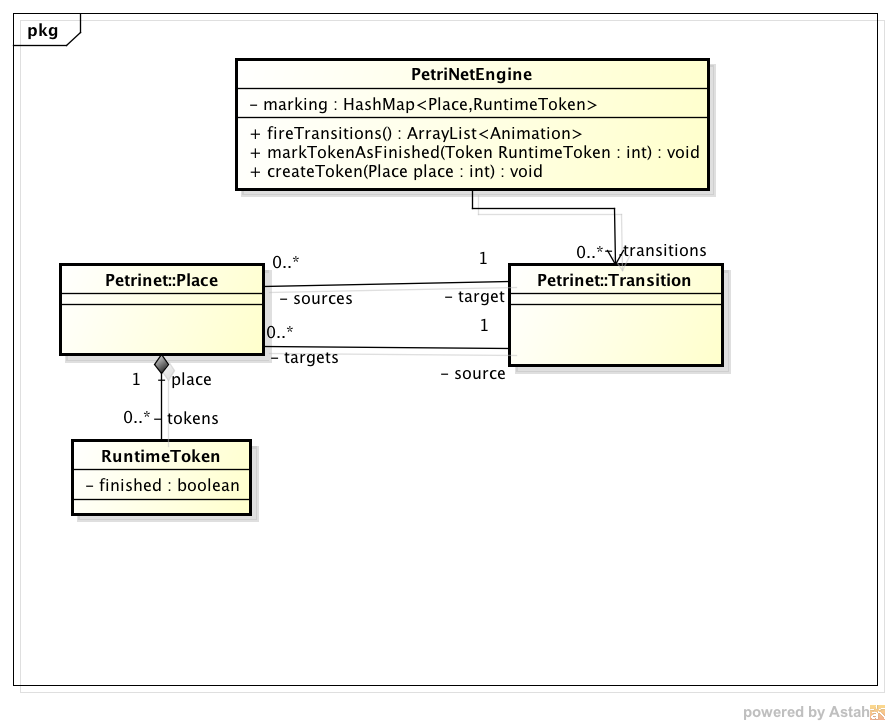
\includegraphics[width=0.8\textwidth]{image/petrinet_engine.png}
  \caption{UML for the Petrinet Engine}
  \label{fig:uml-petrinet-engine}
\end{center}
\end{figure}


 

